\chapter{建模支持工具测试与案例研究}

本章将介绍建模支持工具DDDD的测试与案例研究工作。
介绍了“可视化建模”、“模型校验”以及“模型存储与转化”三个模块的主要功能单元测试;
还以案例的形式演示了工具的完整使用流程,
验证了本文提出的建模支持工具满足开发人员和架构师的战术建模需求。


\section{建模支持工具测试}

本小节主要介绍对建模支持工具的功能测试和性能测试。
主要对工具的三个模块进行测试,
测试的功能主要包括:“可视化建模”、“建模约束校验”、“模型存储”以及“生成项目”。
对“可视化建模”功能进行单元测试,验证建模支持工具是否支持灵活易用的建模过程;
对“建模约束校验”功能进行单元测试,验证建模支持工具是否支持对建模结果正确性和规范性的保障;
对“模型存储”和“生成项目”功能进行单元测试,
验证建模支持工具是否支持模型的保存、复用和扩展使用,
最后对支持主要功能的后端接口进行了性能测试。

进行单元测试时,主要针对实现功能的关键接口进行测试。
涉及前后端交互的部分均以Postman\footnote{Postman工具主页:https://www.postman.com}工具为辅助,
采取JSON格式进行数据传输,代替实际项目中以抽象类封装的数据。
进行性能测试时,以脚本形式对接口进行多次访问,统计接口的平均响应时间。

\subsection{可视化建模测试}

表\ref{testcase1}是对“可视化建模”进行测试的测试用例具体描述。
通过输入一系列鼠标拖拽操作进行测试,
测试的接口是实现绘制图形的核心接口“Draw.addCell”。
测试目的是验证建模支持工具的“可视化建模”功能。
单元测试首先使用拖拽图形的方式进行“实体类”的绘制,
并双击“实体类”修改名称;
然后拖拽图形进行“值对象类”的绘制,并双击修改名称;
最后,进行“实体类”和“值对象类”之间的连线绘制。

测试结果为建模结果的图像表示。
对“可视化建模”进行测试的结果输出如图\ref{Ftestcase1}所示,
该图展示了成功绘制“实体类”和“值对象类”的图形建模结果,
结果表明“可视化建模”可以支持正常建模。

{\footnotesize
\begin{longtable}[h]{m{80pt}|m{305pt}}
    \caption[可视化建模测试用例]{可视化建模测试用例} \label{testcase1} \\
        \hline  
        ID&TC1\\
        \hline
        测试目标&可视化建模实体与值对象,并建立连接\\
        \hline
        测试接口&Draw.addCell\\
        \hline
        前置条件&工具画布初始化正常\\
        \hline
        输入&(1)拖拽“实体类”,绘制在画布中,并修改实体名为“Student”,唯一标识为“ID:String”;
            \newline(2)拖拽“值对象类”,绘制在画布中,并修改值对象名为“Book”;
            \newline(3)建立实体到值对象的连接。\\
        \hline
        预期输出&包含实体和值对象的图形化建模结果\\
        \hline  

    \end{longtable} 
}
    \begin{figure}[!htbp] %figure环境,h默认参数是可以浮动,不是固定在当前位置。如果要不浮动,你就可以使用大写float宏包的H参数,固定图片在当前位置,禁止浮动。
        \centering %使图片居中显示
        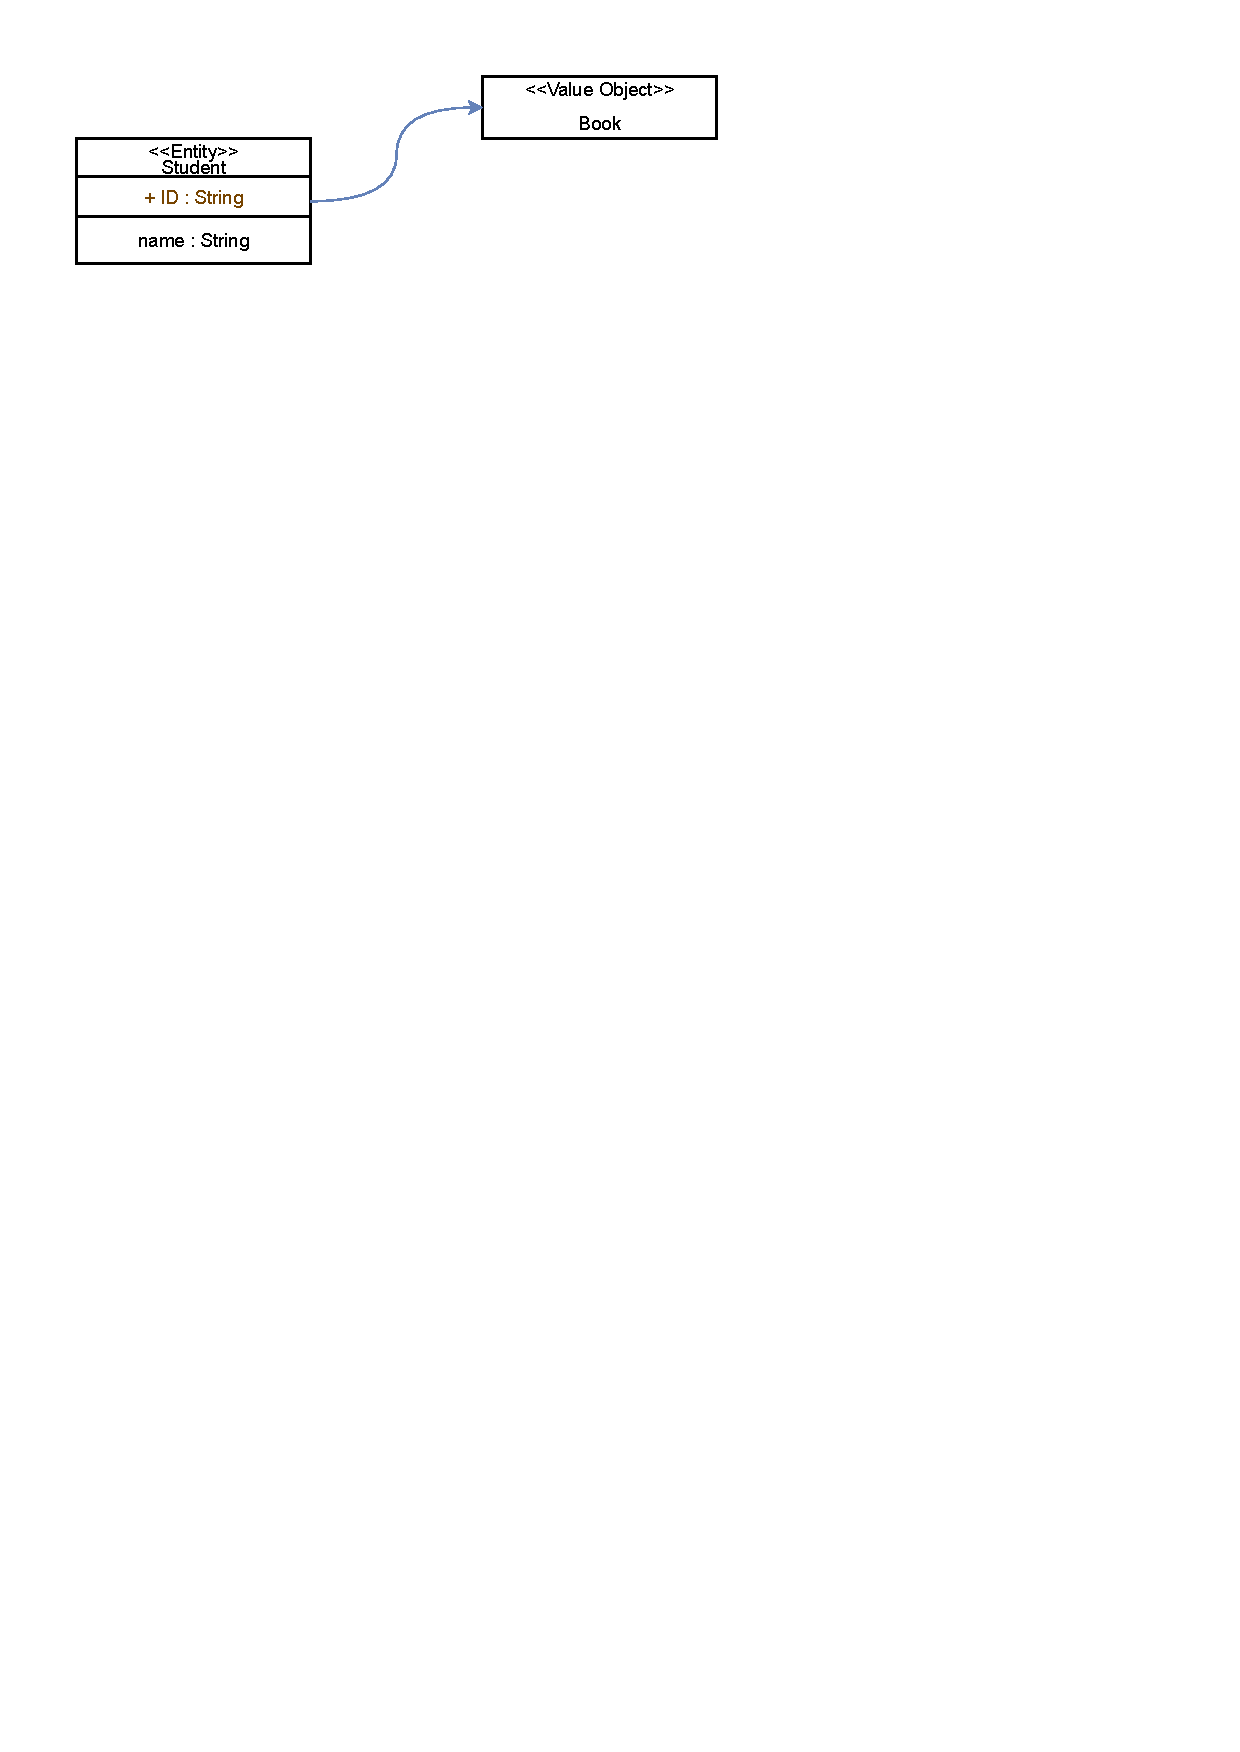
\includegraphics[width=0.8\textwidth]{FIGs/chapter5/Ftestcase1.pdf} %中括号中的参数是设置图片充满文档的大小,你也可以使用小数来缩小图片的尺寸。
        \caption{图形化建模测试结果图} %caption是用来给图片加上图题的
        \label{Ftestcase1} %这是添加标签,方便在文章中引用图片。
    \end{figure}%figure环境

\subsection{建模约束校验测试}

表\ref{testcase2}是对“建模约束校验”进行测试的测试用例具体描述。
输入为包含未连接任何对象的“资源库类”的建模结果,
测试的接口是实现“建模约束校验”的核心接口“PatternData.validatio”。
测试目的是验证对“资源库类”的“建模约束校验”功能。

由于表\ref{stereotypeconstraint}中的约束C12规定,
本次测试结果为校验失败,具体的结果如图\ref{Ftestcase2}所示,
以弹窗形式输出校验警告信息和修改提示。
结果表明“建模约束校验”功能正常实现。

{\footnotesize
\begin{longtable}[h]{m{80pt}|m{305pt}}
    \caption[建模约束校验测试用例]{建模约束校验测试用例} \label{testcase2} \\
        \hline  
        ID&TC2\\
        \hline
        测试目标&正确检测图形化建模约束问题,给出警告提示\\
        \hline
        测试接口&PatternData.validation\\
        \hline
        前置条件&工具画布初始化正常\\
        \hline
        输入& 包含未连接任何对象的“资源库类”的建模结果\\
        \hline
        预期输出& 校验失败信息“请给Repository连接一个它所存储的实体(或聚合根)”\\
        \hline  
\end{longtable} 

}
    \begin{figure}[h] %figure环境,h默认参数是可以浮动,不是固定在当前位置。如果要不浮动,你就可以使用大写float宏包的H参数,固定图片在当前位置,禁止浮动。
        \centering %使图片居中显示
        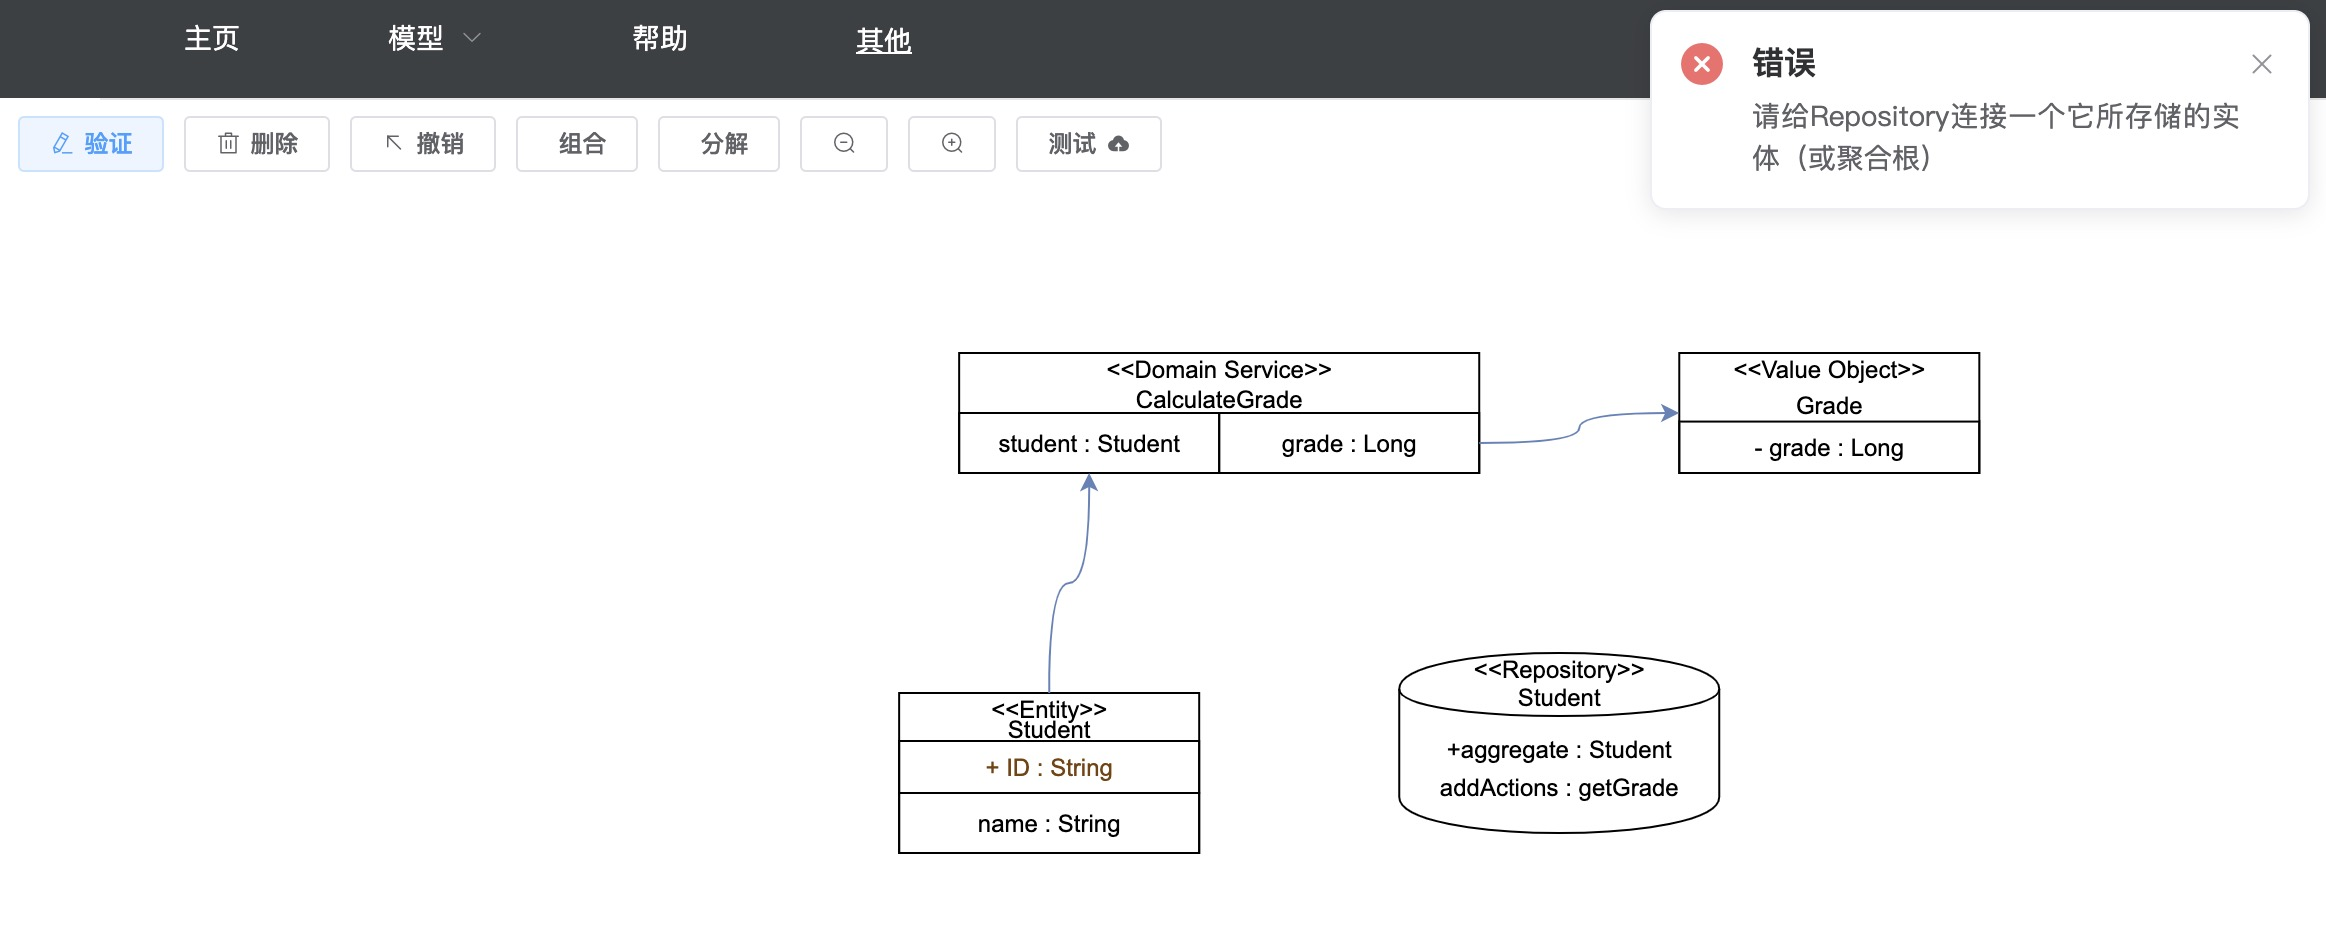
\includegraphics[width=0.8\textwidth]{FIGs/chapter5/Ftestcase2.jpg} %中括号中的参数是设置图片充满文档的大小,你也可以使用小数来缩小图片的尺寸。
        \caption{建模约束校验测试结果图} %caption是用来给图片加上图题的
        \label{Ftestcase2} %这是添加标签,方便在文章中引用图片。
    \end{figure}%figure环境


\subsection{模型存储测试}

表\ref{testcase3}是对“模型存储”进行测试的测试用例具体描述。
输入为模型名称以及模型XML格式文件,
测试的接口是实现“模型存储”的核心接口“ModelRepository.saveModels”。
测试目的为验证模型的“保存”功能。

数据库初始化正常且网络连接通畅,
模型存储测试成功,并可以从数据库中检索出模型,绘制在画布上。
结果表明“模型存储”功能实现正常。

{\footnotesize
\begin{longtable}[h]{m{80pt}|m{305pt}}
    \caption[模型存储测试用例]{模型存储测试用例} \label{testcase3} \\
        \hline
        ID&TC3\\
        \hline
        测试目标&正确存储模型,并能从模型数据库中检索重建模型\\
        \hline
        测试接口&ModelRepository.saveModels\\
        \hline
        前置条件&数据库初始化正常,网络连接通畅\\
        \hline
        输入& 模型名称\\
        \hline
        预期输出& 保存成功提示,成功从数据库中检索模型并重建模型\\
        \hline 

\end{longtable} 
}

\subsection{生成项目测试}

表\ref{testcase4}是对“生成项目”进行测试的测试用例具体描述。
输入为图形化建模结果,
测试的接口是实现“生成框架项目”功能的核心接口“ModelRepository.generateModels”。
测试目的为验证根据建模结果“生成框架项目”的功能。

测试结果为弹出生成项目成功的提示窗口,
并可以在指定文件目录下访问项目文件,
项目文件结构符合领域驱动设计战术建模规范。
结果表明“生成项目”功能实现正常。

{\footnotesize
\begin{longtable}[h]{m{80pt}|m{305pt}}
    \caption[生成项目测试用例]{生成项目测试用例} \label{testcase4} \\
        \hline  
        ID&TC4\\
        \hline
        测试目标&根据图形化建模结果生成框架项目\\
        \hline
        测试接口&ModelRepository.generateModels\\
        \hline
        前置条件&无\\
        \hline
        输入& 图形化建模结果\\
        \hline
        预期输出& 指定文件路径下的框架项目文件包\\
        \hline
\end{longtable} 
}

\subsection{性能测试}

性能测试部分主要针对“模型存储与转化”功能中的核心接口进行测试。
测试环境如表\ref{testcase5}所示,描述了测试环境服务器的具体配置,
将ElasticSearch部署至该测试环境中进行测试。

{\footnotesize
\begin{longtable}[h]{m{100pt}|m{285pt}}
    \caption[测试环境]{测试环境} \label{testcase5} \\
        \hline  
        配置项&描述\\
        \hline
        操作系统&CentOS 7.6 64位\\
        \hline
        CPU&Intel(R) Xeon(R) Platinum 8269CY,4核,2.5 GHz/3.2 GHz\\
        \hline
        内存&8G\\
        \hline
        Java版本& OpenJDK 1.8.0 181\\
        \hline
        ElasticSearch版本& 7.11.1\\
        \hline
\end{longtable} 
}

建模支持工具的所有模块中,
“模型存储与转化”模块前后端交互频繁,
需要经常请求持久化设施,
而其他模块的前后端交互很少,
几乎不需要考虑性能问题。
故主要对“模型存储与转化”模块的接口进行性能测试。
请求持久化设施会在网络上发生耗时的数据传输操作,
所以响应时间(Response Time,RT)是衡量接口性能的核心指标,
性能测试通过编写脚本对每个核心接口进行50次请求,并统计平均响应时间。
具体测试结果如表\ref{testcase6}所示,
展示了测试接口的平均响应时间,
测试的接口包括保存模型的“saveModel”接口,
查询模型的“getModels”接口,
删除模型的“deleteModel”接口,
以及搜索模型的“getModelByKeyword”接口。
表中平均响应时间说明后端接口反馈迅速,
基本满足性能需求。


{\footnotesize
\begin{longtable}[]{m{130pt}|m{100pt}|m{140pt}}
    \caption[接口性能测试]{接口性能测试} \label{testcase6} \\
        \hline  
        接口名&请求类型&平均响应时间\\
        \hline
        saveModel&PUT&50ms\\
        \hline
        getModels&GET&21ms\\
        \hline
        deleteModel&DELETE&13ms\\
        \hline
        getModelByKeyword&GET&18ms\\
        \hline
\end{longtable} 
}

\section{案例研究}

本小节对本文提出的战术建模支持方法及工具进行案例研究。
通过案例演示使用支持工具进行建模的完整过程,
来验证该建模支持方法和工具是否能够提供灵活易用的建模支持,
提高建模效率;
是否能够保证建模结果的标准化、规范化;
以及是否能够满足建模结果的持久性、可复用性和扩展应用。

为验证本工具能够支持战术建模整个流程,本文以Vaughn Vernon的
《实现领域驱动设计》\cite{vernon2013implementing}
中的企业协作软件系统CollabOvation为研究案例展开验证。

SaaSOvation是一家企业办公软件提供商,
CollabOvation是由SaaSOvation公司开发的一款企业协作(Collaboration)软件,
并且加入社交网络的功能。
该产品的功能包括论坛、共享日历、博客、即时消息、wiki、留言板、文档管理、通知和提醒、活动跟踪和RSS等。
所有协作工具都旨在满足企业服务的需求,帮助他们在项目中提高效率。
CollabOvation项目启动后,项目中的一些有经验的开发人员采用领域驱动设计
将项目划分为协作上下文、身份与访问上下文和敏捷项目上下文,
具体项目代码已发布到GitHub\footnote{IDDD-Samples代码仓库地址:https://github.com/VaughnVernon/IDDD$_Samples/$}代码仓库。
案例研究将CollabOvation的身份与访问上下文作为业务范围,
进行战术建模。案例研究验证过程包括使用建模支持工具进行标准化战术建模的五个具体步骤,
并给出平台截图展示。



\subsection{验证步骤}

本小节将对建模支持方法及工具进行验证,
首先验证可视化建模能否支撑含有复杂设计的战术建模,
满足图形化的建模基本需求;
其次验证对精细化建模的支持程度,能否正确识别建模中不规范的操作,
并给予相应的提示;
最后验证建模结果的存储与转化使用,
能否正确存储建模结果并生成框架项目指导编码工作。

Vaughn Vernon在《实现领域驱动设计》\cite{vernon2013implementing}中
已经详细介绍了项目的背景和需求,
但没有进一步细化划分出的限界上下文,
以下的验证步骤的目的(也是本案例研究的目的)
在于探究本文所提出的建模支持方法及工具能否支持对所选案例进行战术建模,
具体验证工作步骤如下:

\textbf{步骤一:}开发人员通过工具快速学习战术建模相关概念知识;

\textbf{步骤二:}开发人员进入可视化建模页面,进行建模;

\textbf{步骤三:}对于不符合战术建模规范的操作,没有通过战术模式约束校验的属性弹出警告提示;

\textbf{步骤四:}建模结果校验通过,将模型导出为XML文件和图片,保存到数据库中,并生成框架项目文件;

\textbf{步骤五:}读取保存的模型文件或数据库中存储的模型,进行二次建模。

\subsection{验证过程}

本小节将依据上一节所述的步骤对支持工具进行演示和验证。

\textbf{步骤一:}点击工具平台首页的“Can I DDD”按钮,进入展示战术建模相关概念知识的帮助页面,
如图\ref{modelknowledge}所示为帮助页面。
该页面帮助开发人员快速了解战术建模相关概念与使用场景,回顾战术建模知识,降低使用工具的门槛。

\begin{figure}[!htbp] %figure环境,h默认参数是可以浮动,不是固定在当前位置。如果要不浮动,你就可以使用大写float宏包的H参数,固定图片在当前位置,禁止浮动。
    \centering %使图片居中显示
    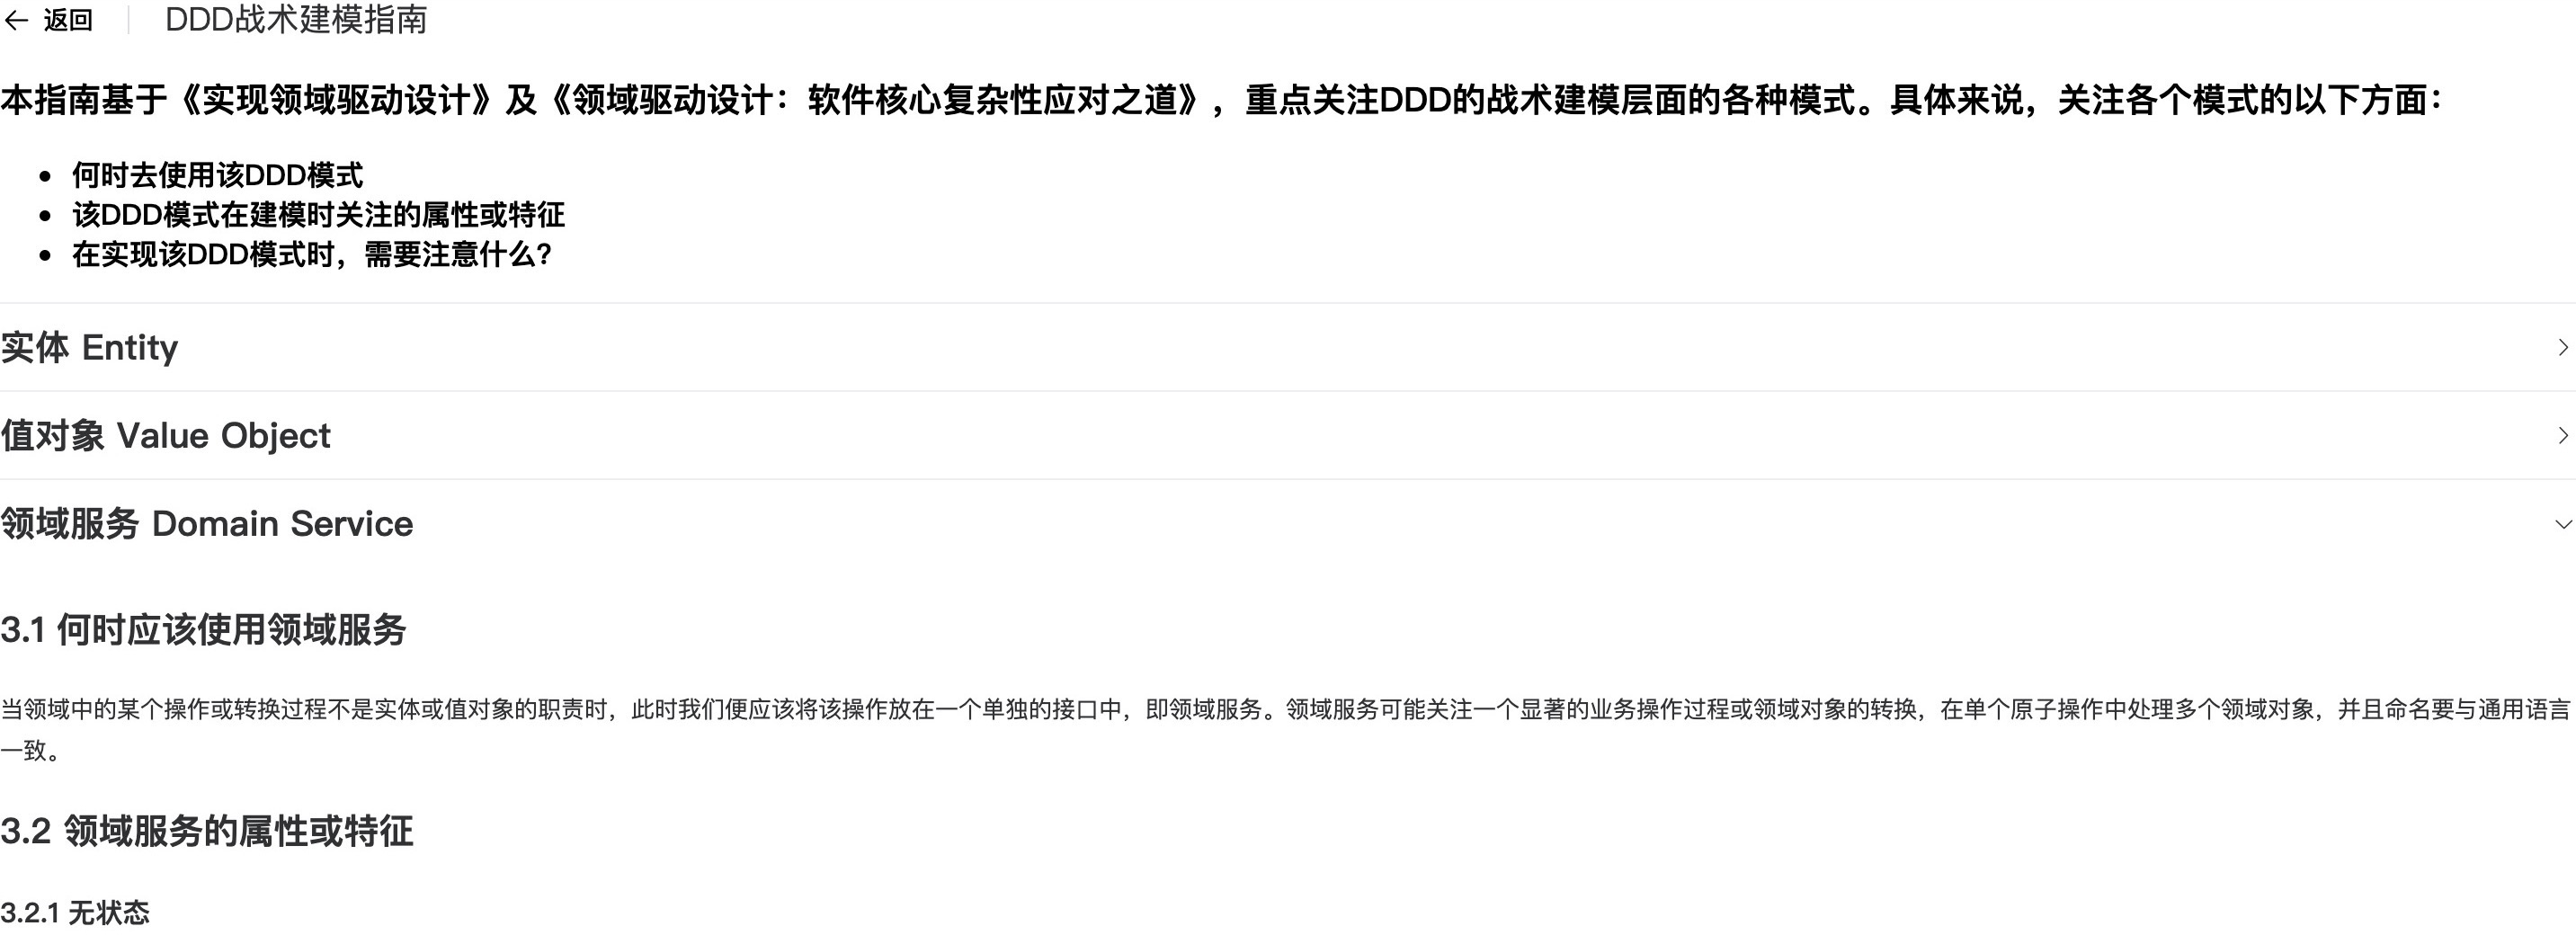
\includegraphics[width=0.8\textwidth]{FIGs/chapter5/modelknowledge.png} %中括号中的参数是设置图片充满文档的大小,你也可以使用小数来缩小图片的尺寸。
    \caption{工具帮助页面图} %caption是用来给图片加上图题的
    \label{modelknowledge} %这是添加标签,方便在文章中引用图片。
\end{figure}%figure环境

\textbf{步骤二:}开发人员或架构师进入可视化建模页面,根据项目背景需求进行战术建模,
由于整个战术建模过程时间跨度长,模型复杂,故仅选择战术建模的一部分进行展示:

\begin{figure}[!htbp] %figure环境,h默认参数是可以浮动,不是固定在当前位置。如果要不浮动,你就可以使用大写float宏包的H参数,固定图片在当前位置,禁止浮动。
    \centering %使图片居中显示
    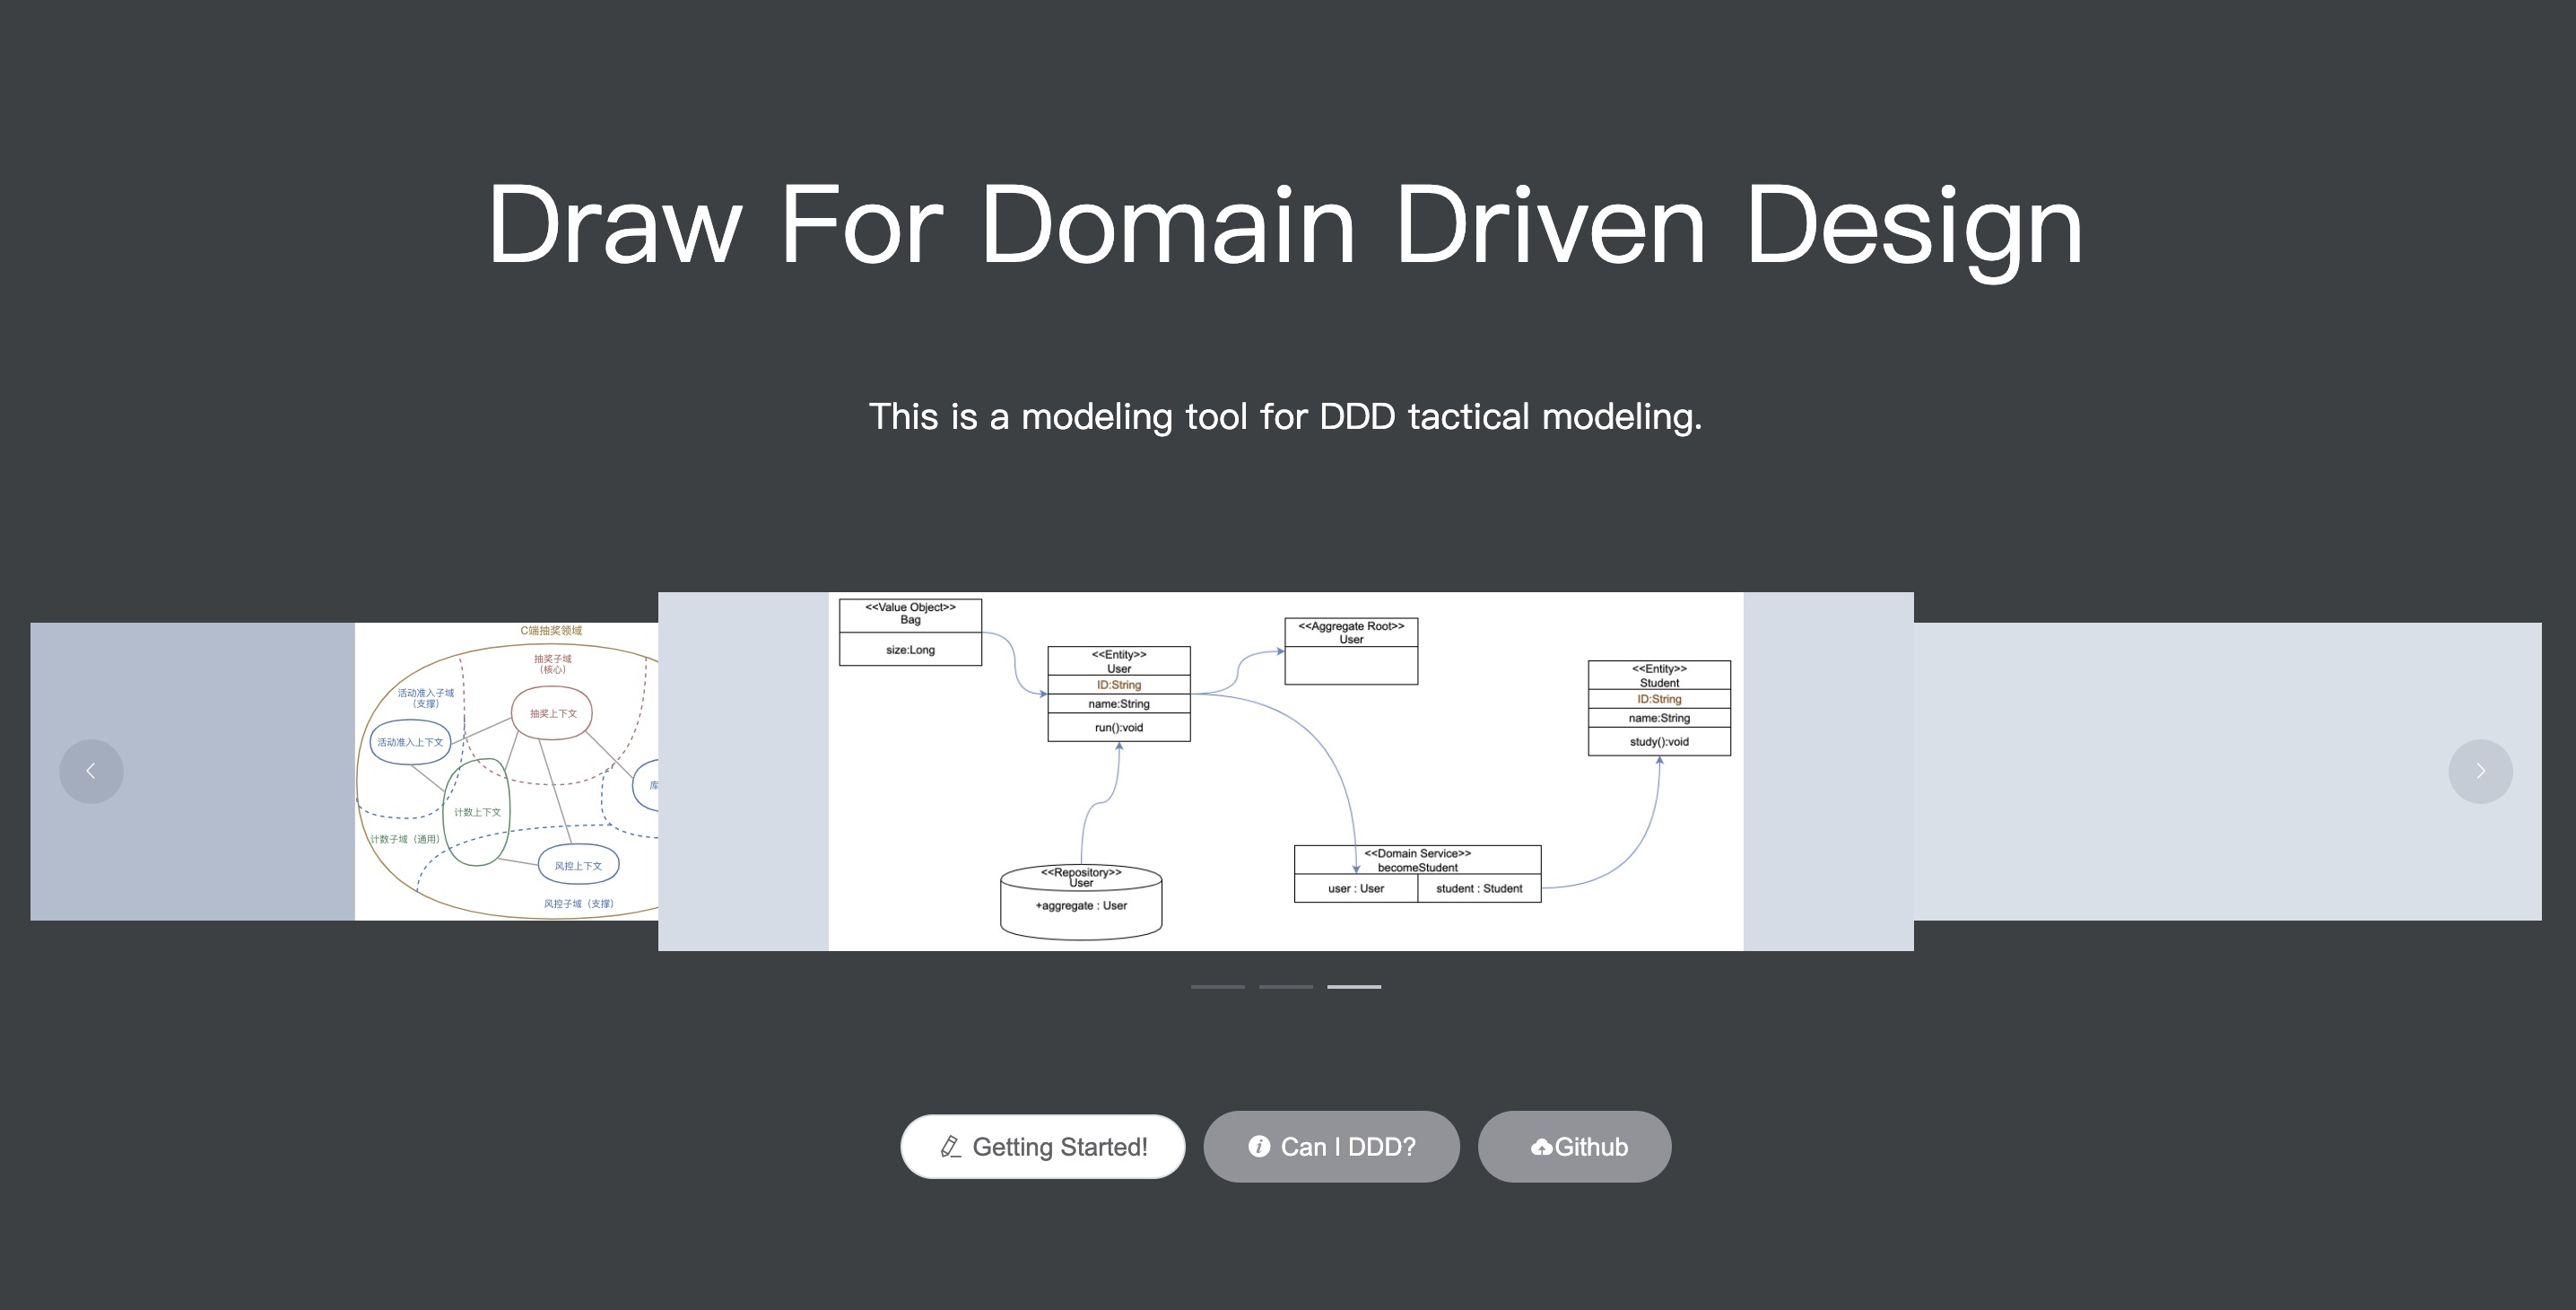
\includegraphics[width=0.8\textwidth]{FIGs/chapter5/toolhome.png} %中括号中的参数是设置图片充满文档的大小,你也可以使用小数来缩小图片的尺寸。
    \caption{工具主页} %caption是用来给图片加上图题的
    \label{toolhome} %这是添加标签,方便在文章中引用图片。
\end{figure}%figure环境



\begin{enumerate}
    \item 工具主页如图\ref{toolhome}所示,点击“Getting Started!”按钮进入建模页面;
    \item 进入建模页面后,拖动左侧工具栏实体、值对象以及领域事件模式图,
    放在右侧画布合适位置,进行绘制;
    \item 双击需要修改的模式属性,输入文字进行修改;
    \item 点击对象,按住拖动进行对象间连线;
    \item 点击右侧画布菜单按钮,可以对建模操作进行撤销,对画布进行缩放,将建模对象进行组合和删除。
\end{enumerate}
\begin{figure}[!htbp] %figure环境,h默认参数是可以浮动,不是固定在当前位置。如果要不浮动,你就可以使用大写float宏包的H参数,固定图片在当前位置,禁止浮动。
    \centering %使图片居中显示
    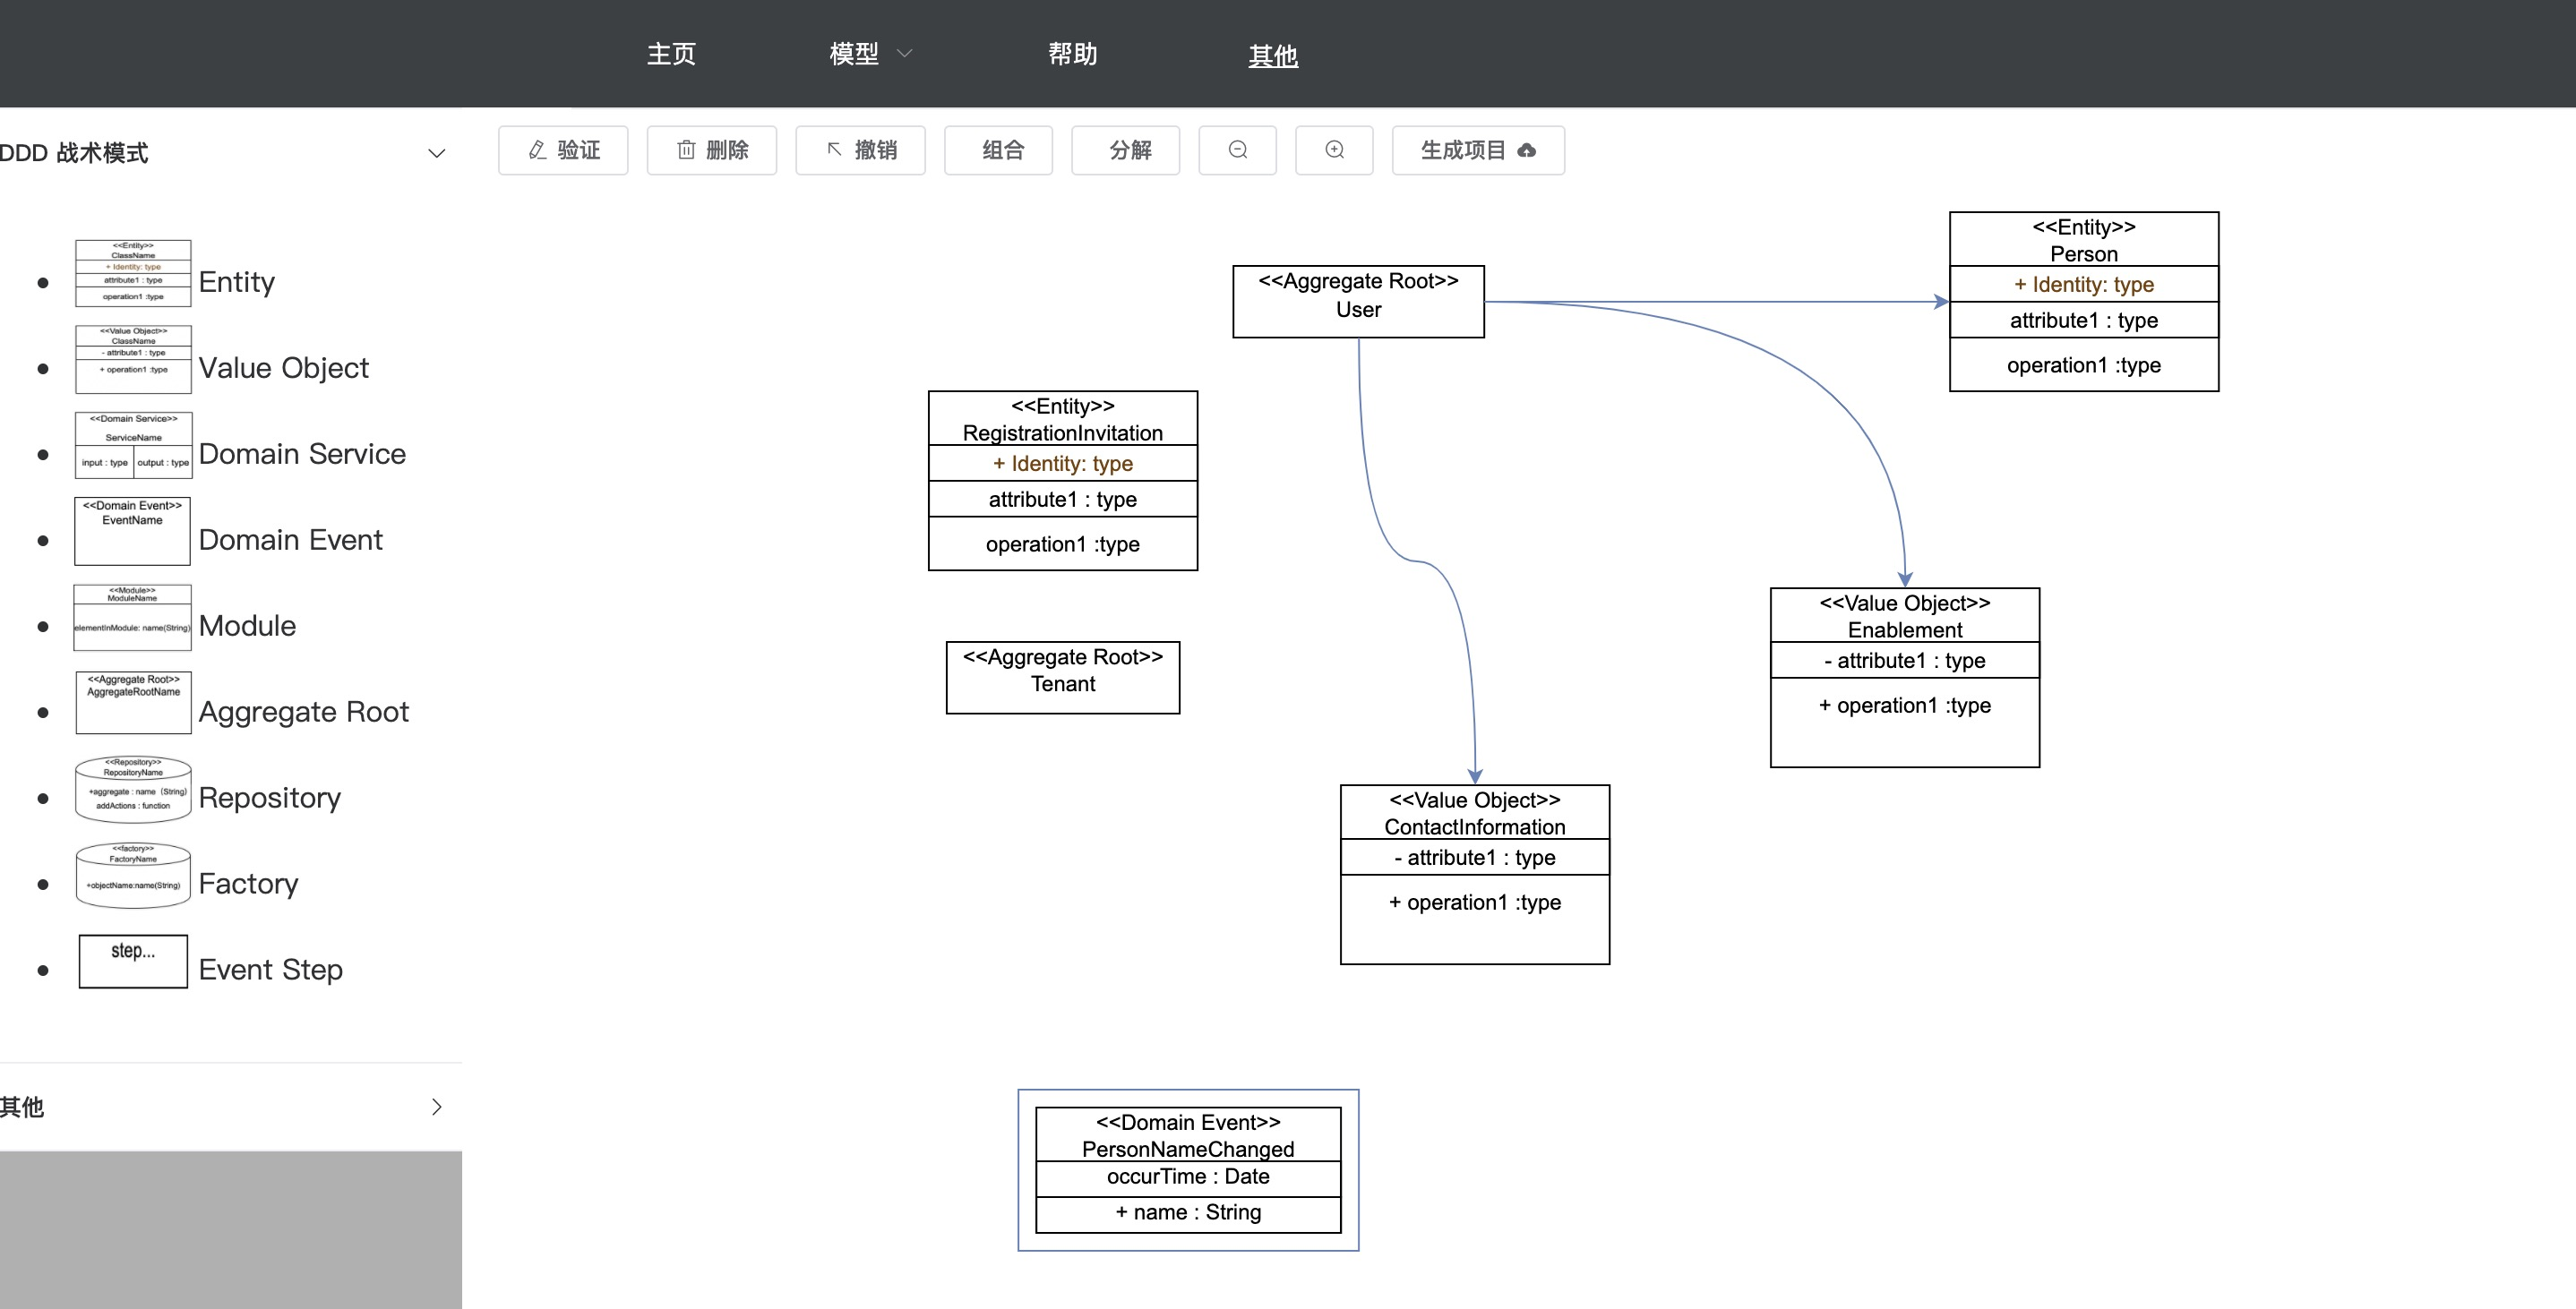
\includegraphics[width=0.8\textwidth]{FIGs/chapter5/drawingmodel.png} %中括号中的参数是设置图片充满文档的大小,你也可以使用小数来缩小图片的尺寸。
    \caption{可视化建模过程} %caption是用来给图片加上图题的
    \label{drawingmodel} %这是添加标签,方便在文章中引用图片。
\end{figure}%figure环境


如图\ref{drawingmodel}所示,展示了上述步骤二的建模过程最终结果。


\textbf{步骤三:}建模时可以对建模结果进行实时校验,校验规则严格按照
本文提出的战术建模支持方法要求,并给出校验结果展示:

\begin{enumerate}
    \item 进行可视化建模时,点击右侧画布菜单按钮“验证”;
    \item 如图\ref{validation}所示,根据当前图形化建模结果,进行约束和规则校验,弹出不符合规范和约束的警告信息。
    
    \begin{figure}[!htbp] %figure环境,h默认参数是可以浮动,不是固定在当前位置。如果要不浮动,你就可以使用大写float宏包的H参数,固定图片在当前位置,禁止浮动。
        \centering %使图片居中显示
        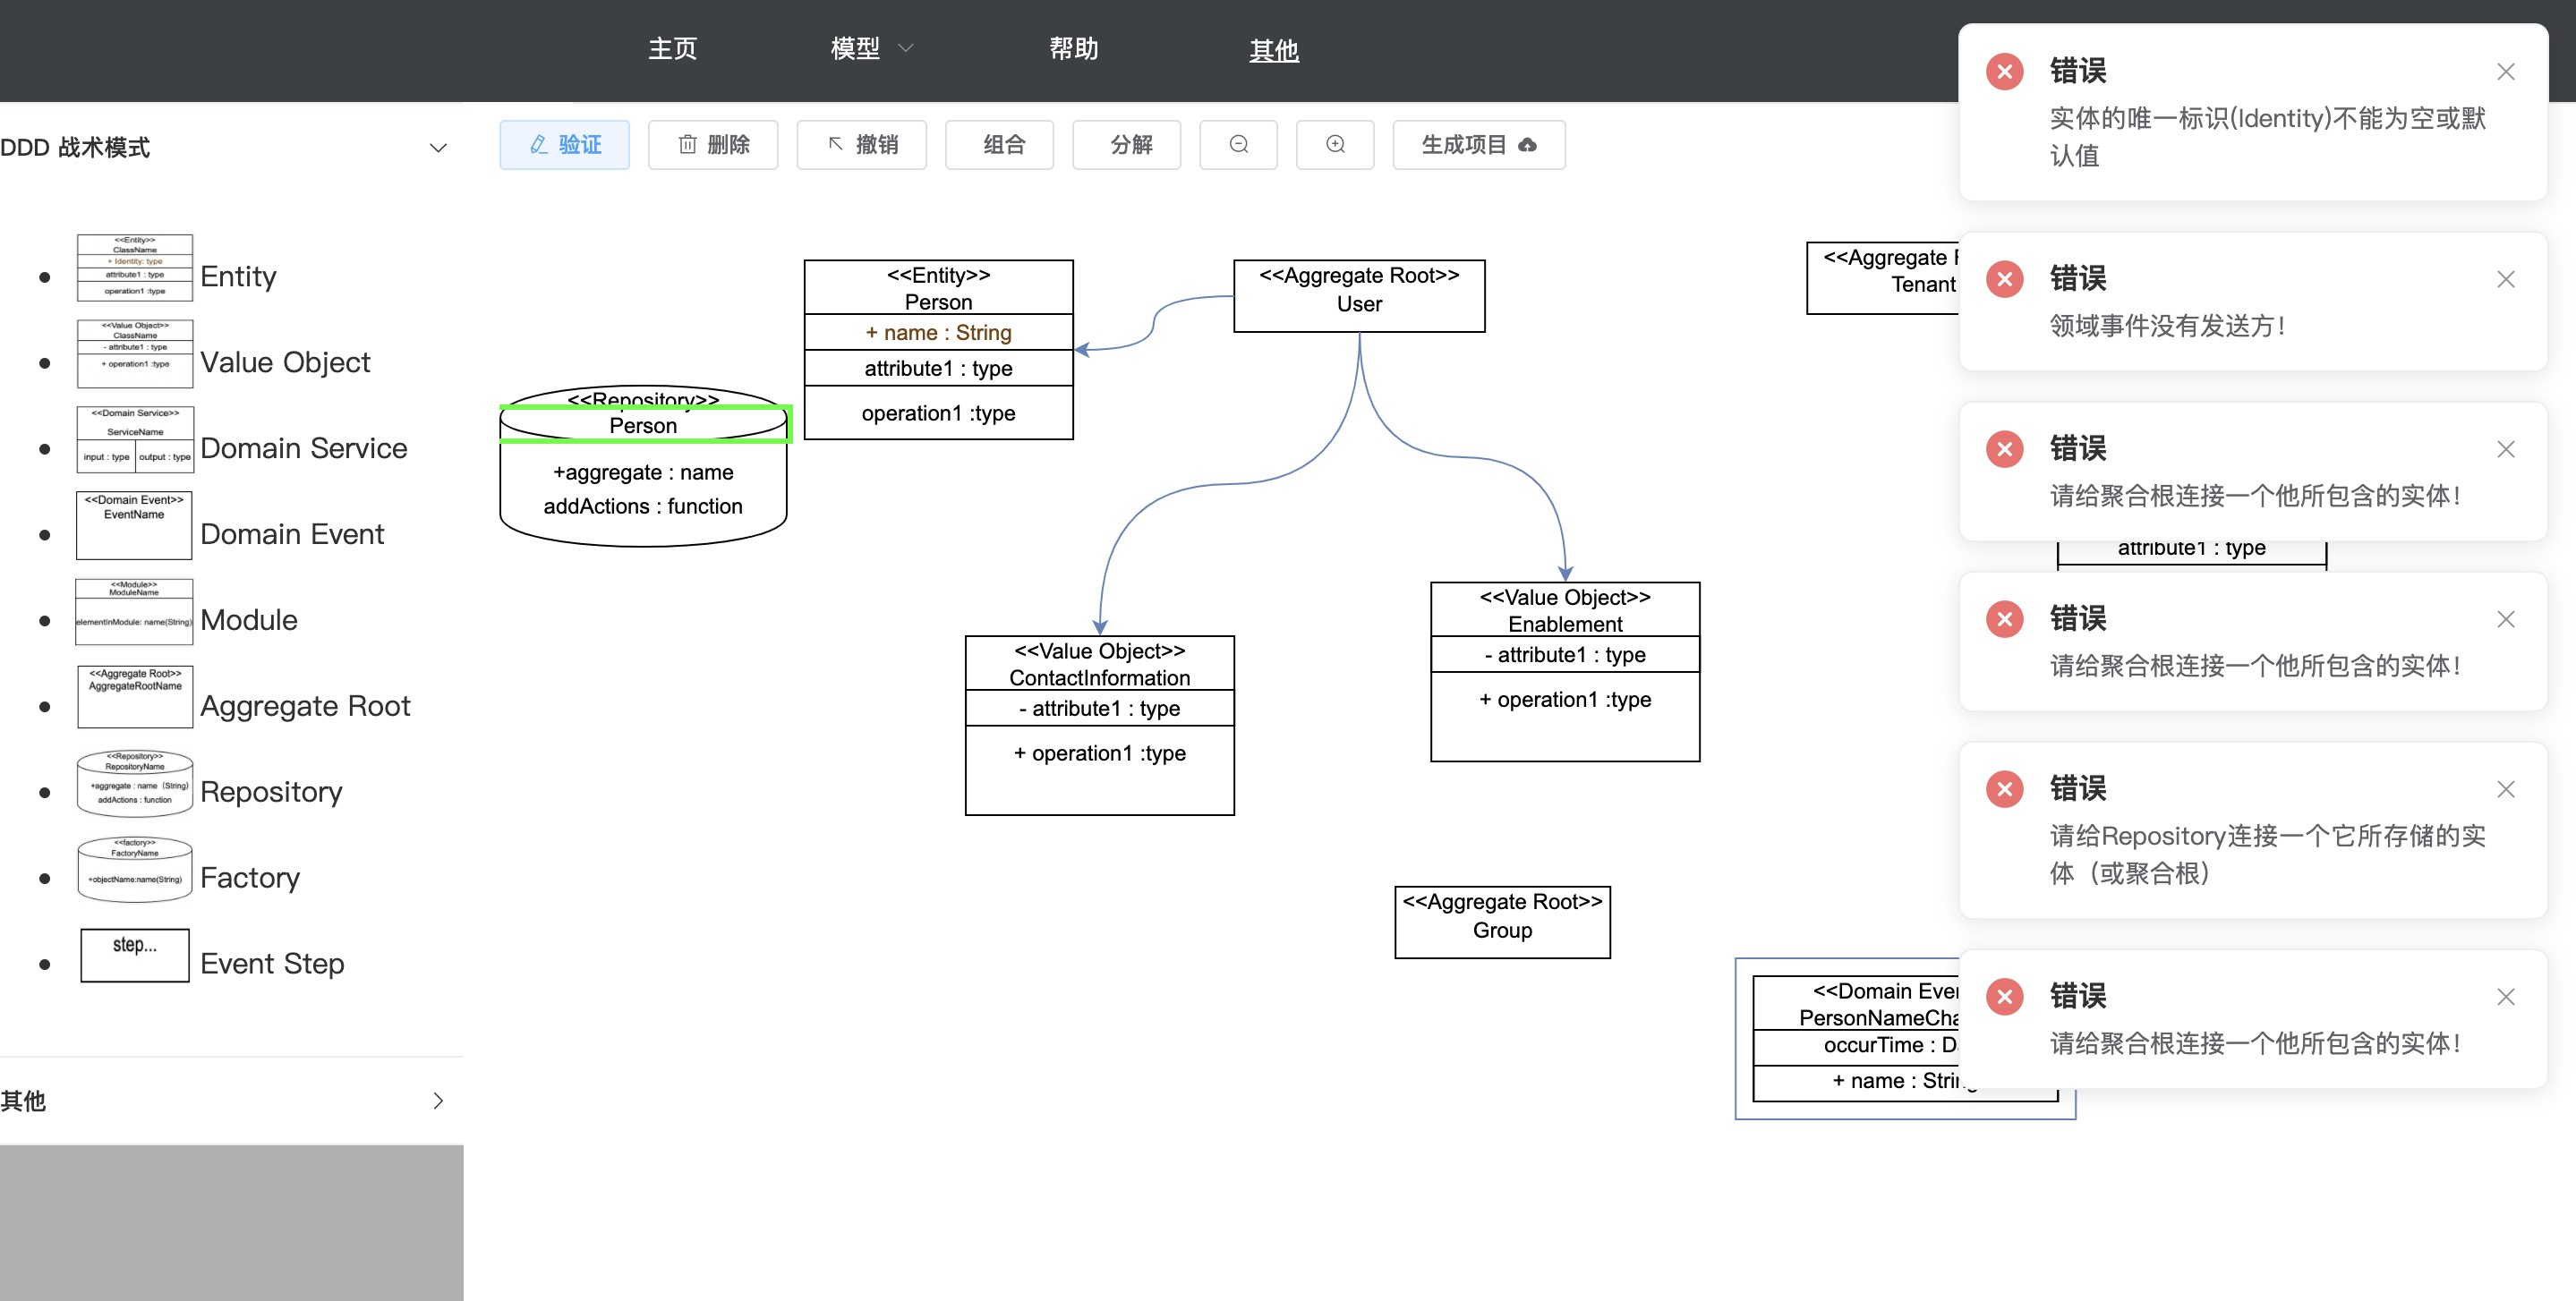
\includegraphics[width=0.8\textwidth]{FIGs/chapter5/validation.png} %中括号中的参数是设置图片充满文档的大小,你也可以使用小数来缩小图片的尺寸。
        \caption{模型校验} %caption是用来给图片加上图题的
        \label{validation} %这是添加标签,方便在文章中引用图片。
    \end{figure}%figure环境
\end{enumerate}

\textbf{步骤四:}选择菜单如图\ref{exportModel}所示,建模完成后,经过校验模型符合规范,可以将模型以XML、图像形式导出,
并存储到数据库中。

\begin{enumerate}
    \item 建模完成,校验通过;
    \item 在菜单中依次选择“模型”、“导出”、“XML格式”,选择保存文件夹;
    \item 在菜单中依次选择“模型”、“导出”、“图像格式”,选择保存文件夹;
    \item 在菜单中依次选择“模型”、“保存模型到数据库”,将模型命名为“userAccess”,点击确定;
    \item 在画布菜单中点击按钮“生成项目”,框架项目文件在指定文件目录中生成。
    \begin{figure}[!htbp] %figure环境,h默认参数是可以浮动,不是固定在当前位置。如果要不浮动,你就可以使用大写float宏包的H参数,固定图片在当前位置,禁止浮动。
        \centering %使图片居中显示
        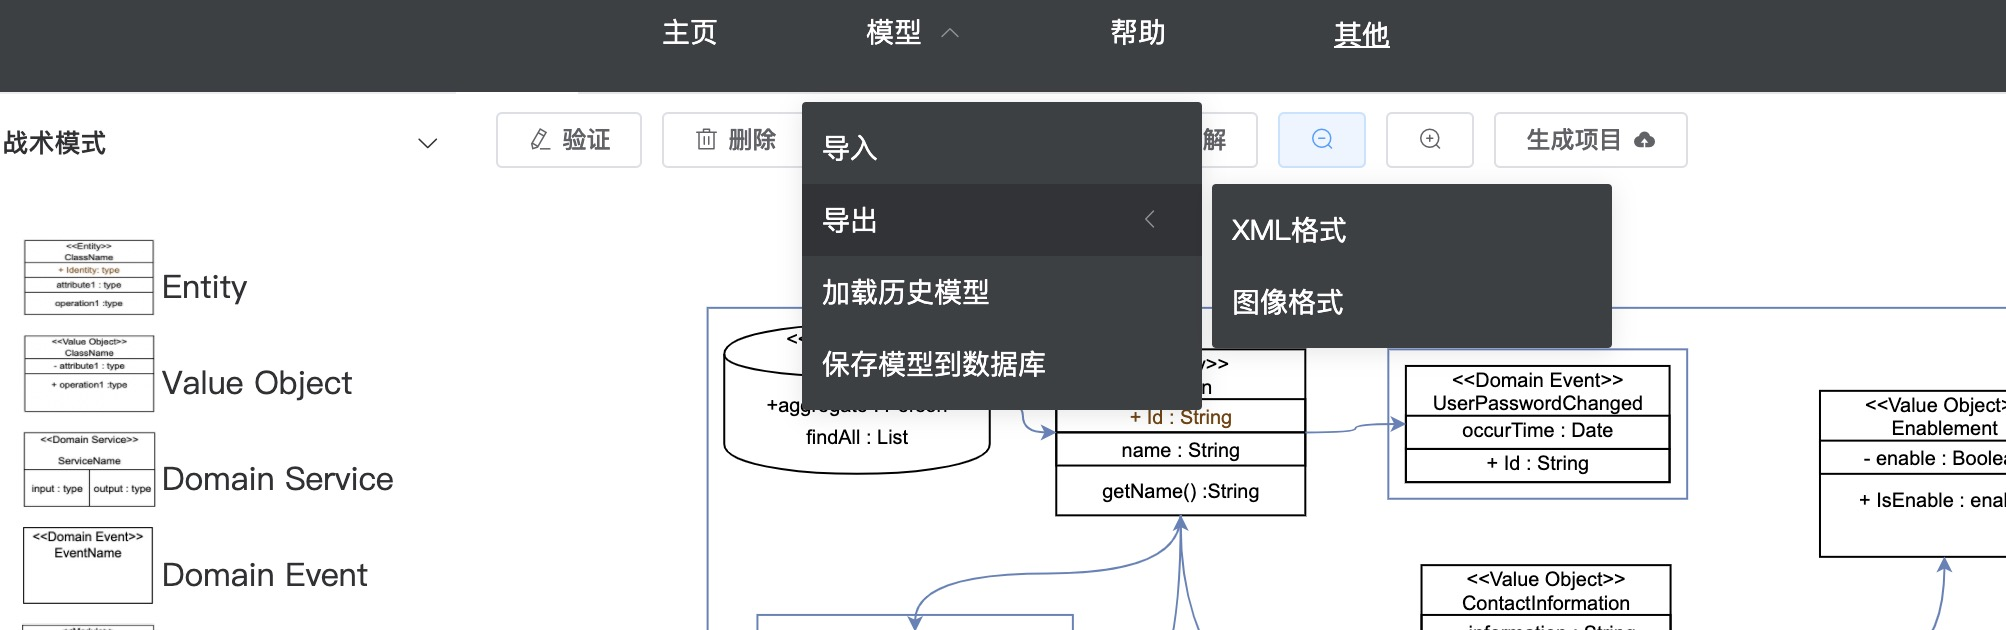
\includegraphics[width=0.8\textwidth]{FIGs/chapter5/exportModel.png} %中括号中的参数是设置图片充满文档的大小,你也可以使用小数来缩小图片的尺寸。
        \caption{保存导出模型} %caption是用来给图片加上图题的
        \label{exportModel} %这是添加标签,方便在文章中引用图片。
    \end{figure}%figure环境
\end{enumerate}

\textbf{步骤五:}再次使用工具时,可以使用“导入”和“加载历史模型”功能,
来重现建模结果,并进行二次建模。
\begin{enumerate}
    \item 在菜单中依次选择“模型”、“加载历史模型”,持久化设施中保存的模型文件列表如图\ref{reloadModel}所示,
    展示了模型名称、创建时间以及操作按钮;

    \begin{figure}[!htbp] %figure环境,h默认参数是可以浮动,不是固定在当前位置。如果要不浮动,你就可以使用大写float宏包的H参数,固定图片在当前位置,禁止浮动。
        \centering %使图片居中显示
        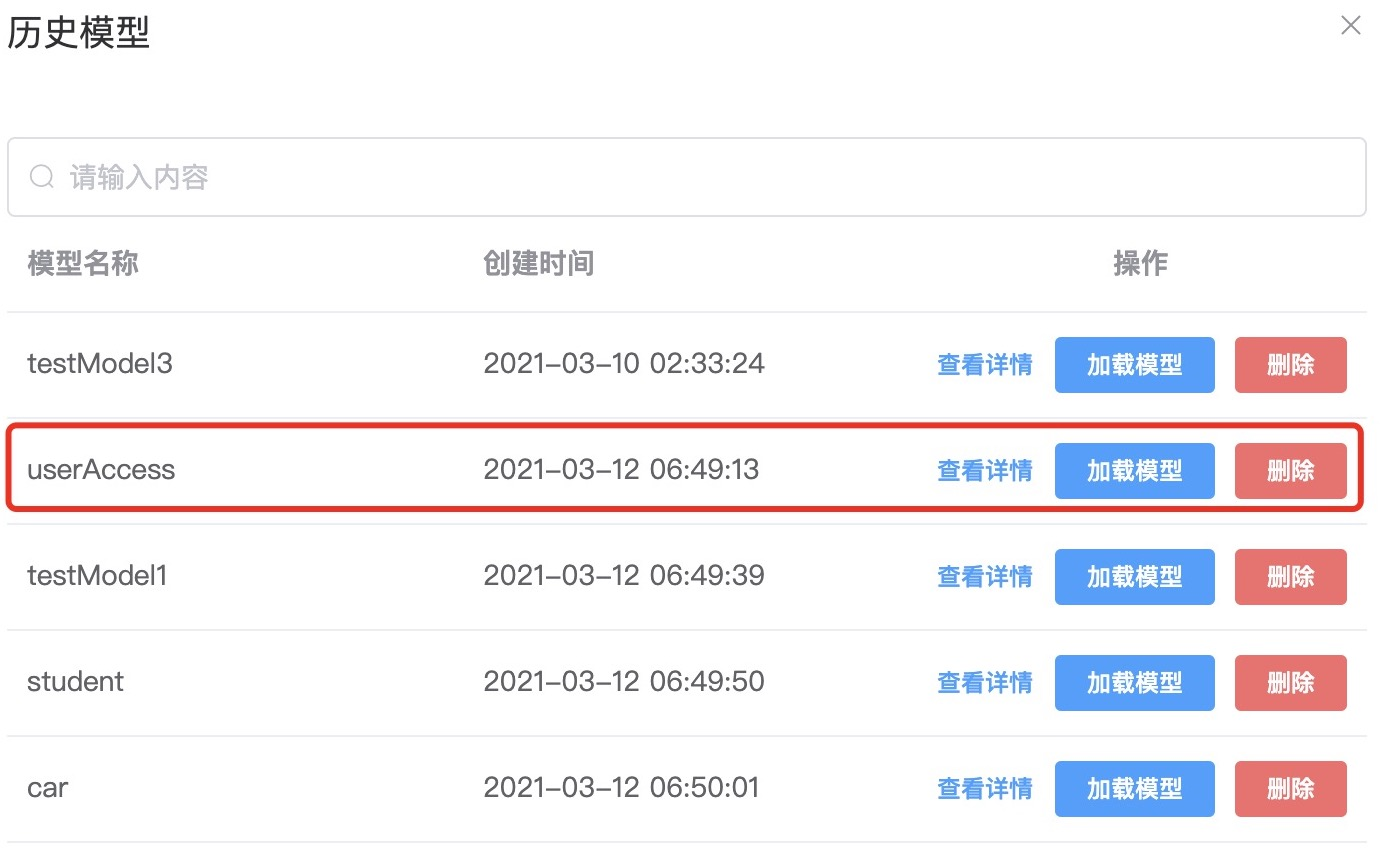
\includegraphics[width=0.8\textwidth]{FIGs/chapter5/reloadModel.png} %中括号中的参数是设置图片充满文档的大小,你也可以使用小数来缩小图片的尺寸。
        \caption{加载历史模型} %caption是用来给图片加上图题的
        \label{reloadModel} %这是添加标签,方便在文章中引用图片。
    \end{figure}%figure环境

    \item 选择想要加载的模型,点击“加载模型”按钮,画布中将绘制出模型;
    \item 加载的历史模型如图\ref{modelResult}所示,可以对历史模型进行新的操作。
\end{enumerate}

\begin{figure}[!htbp] %figure环境,h默认参数是可以浮动,不是固定在当前位置。如果要不浮动,你就可以使用大写float宏包的H参数,固定图片在当前位置,禁止浮动。
    \centering %使图片居中显示
    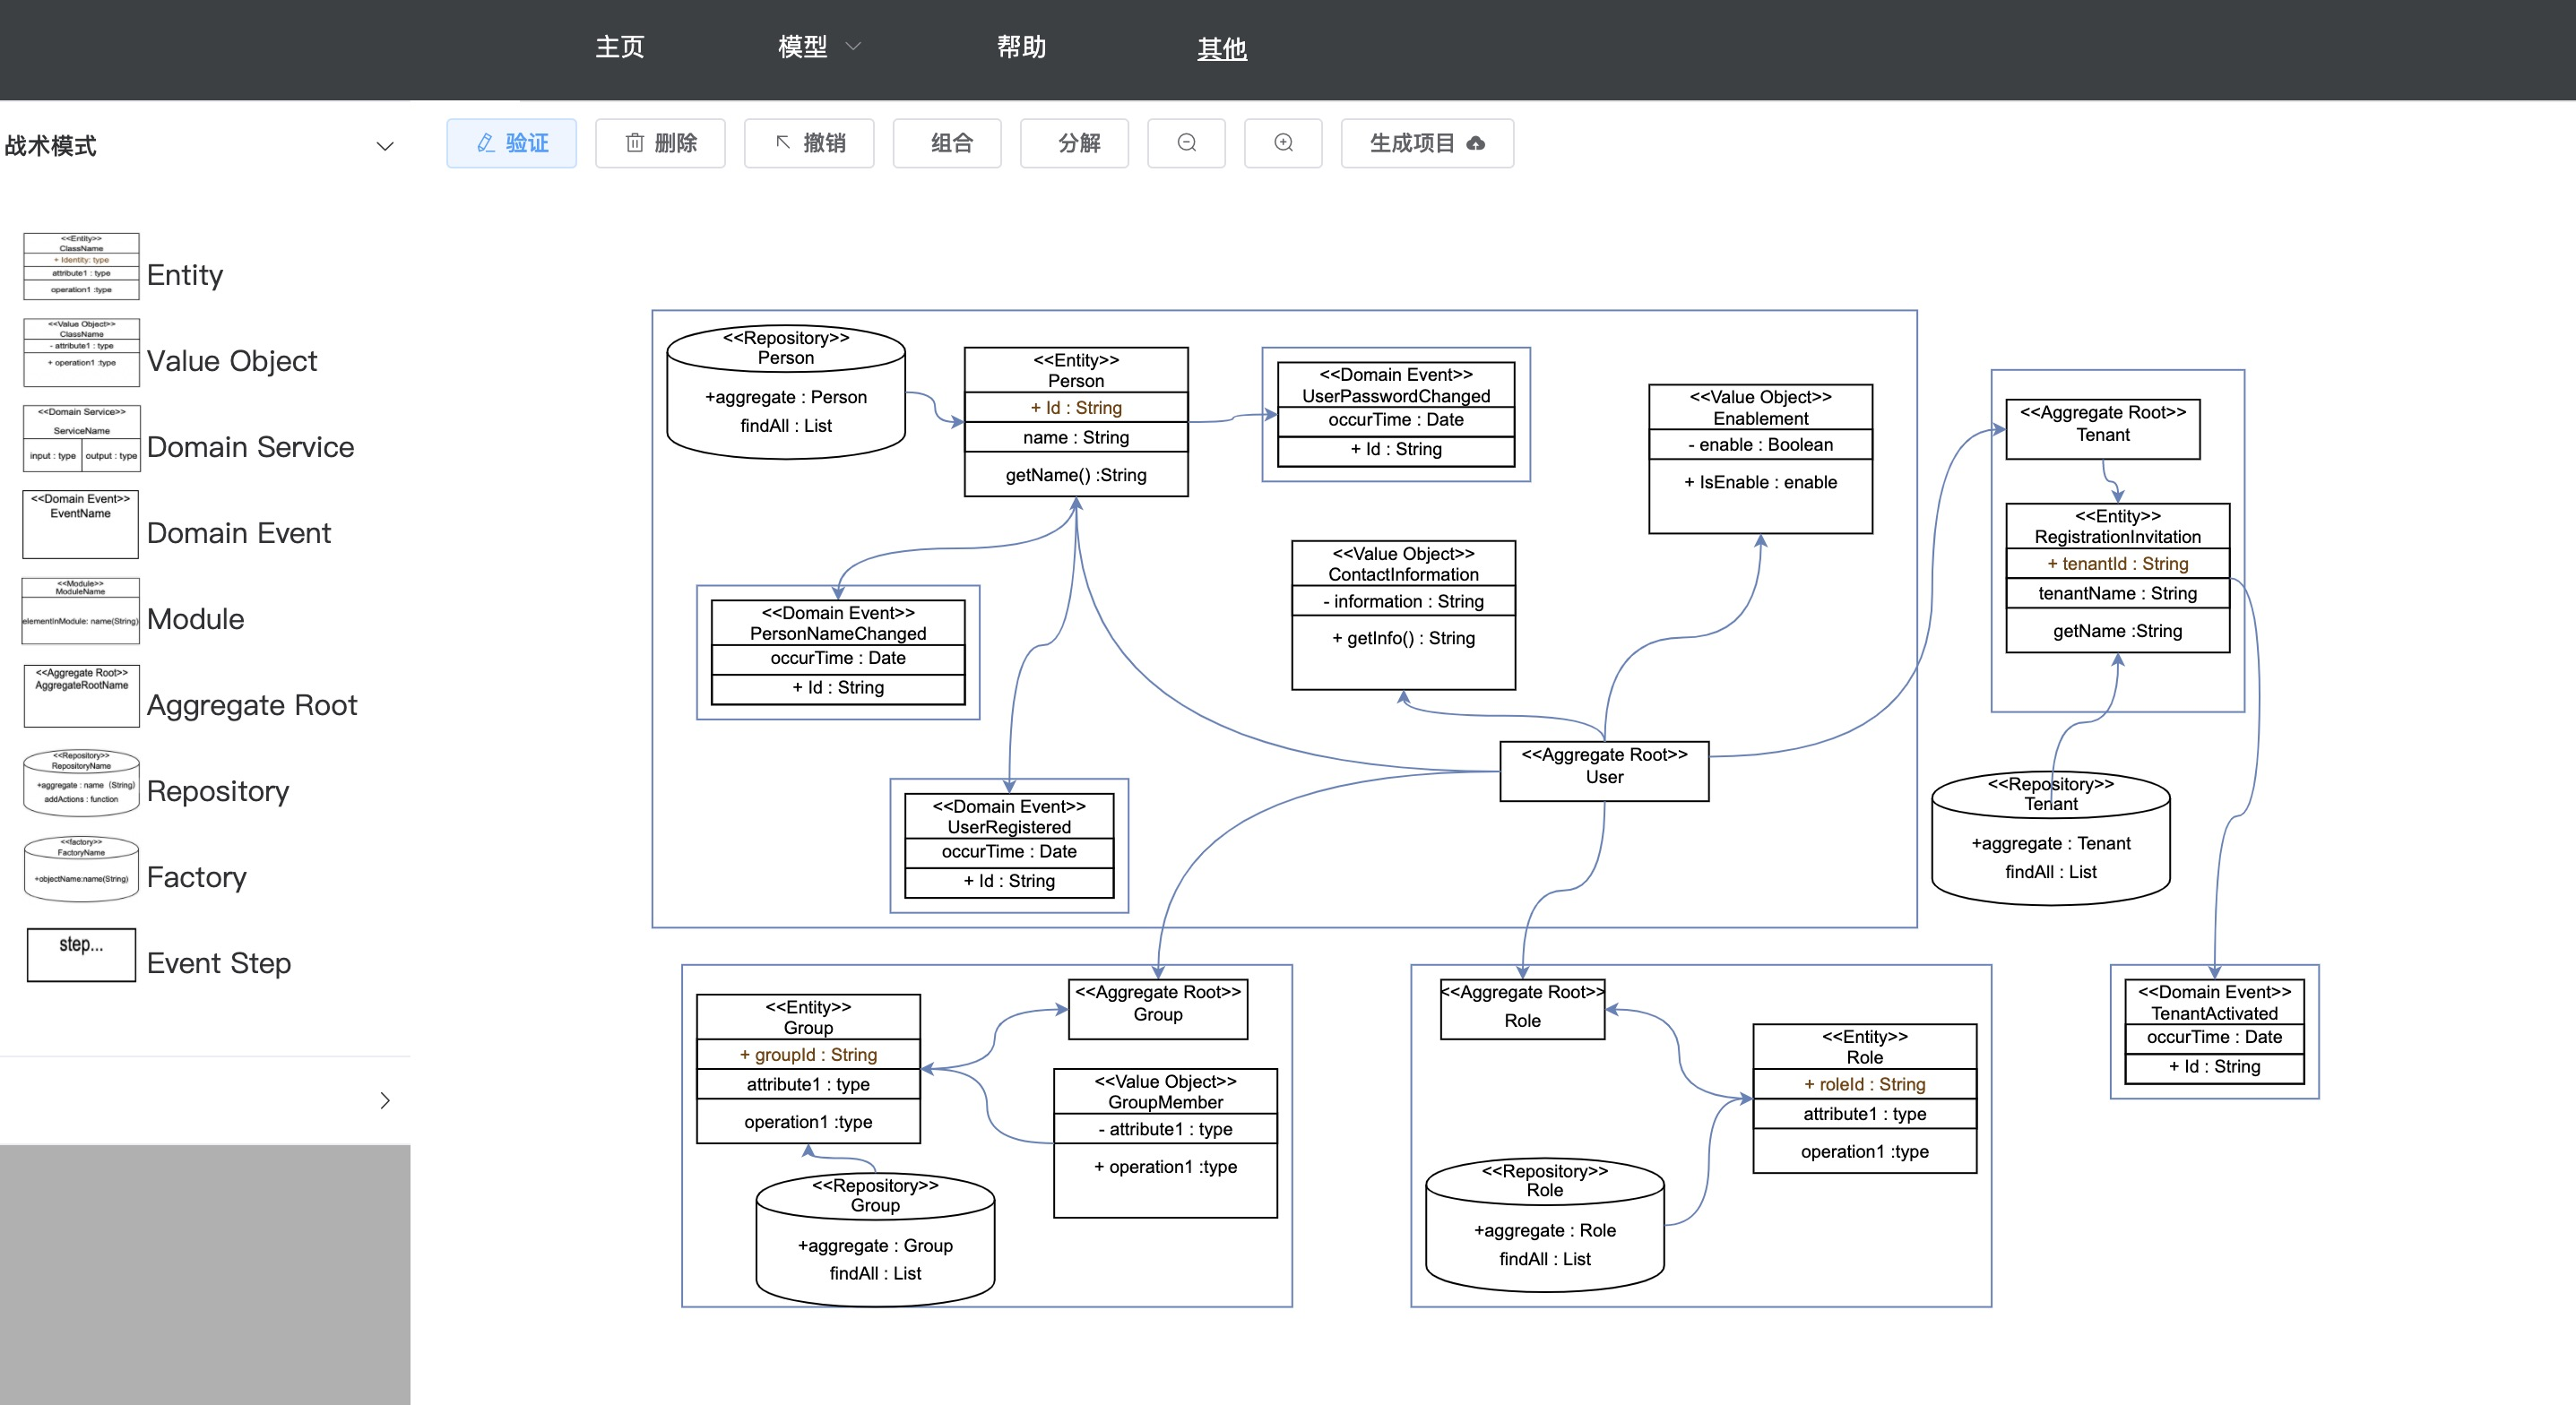
\includegraphics[width=0.8\textwidth]{FIGs/chapter5/modelResult.png} %中括号中的参数是设置图片充满文档的大小,你也可以使用小数来缩小图片的尺寸。
    \caption{建模结果图} %caption是用来给图片加上图题的
    \label{modelResult} %这是添加标签,方便在文章中引用图片。
\end{figure}%figure环境

通过上述五个步骤的验证,得到验证结果如表\ref{validationresult}所示,
表格展示了每个步骤对应的功能需求和验证的结果。
以上步骤和得到的结果表明,
提出的建模支持方法及工具达到了以下效果。
第一,实现了可视化战术建模,使建模过程更加高效灵活;
第二,对建模结果进行约束验证,来判断是否符合战术建模需要遵守的规则,
解决了战术建模阶段流程化与标准化的规范性问题;
第三,可以将建模结果进行存储,方便下次访问,
并提供根据建模结果生成框架项目的扩展功能,
提高了建模结果的可复用性和扩展性。

{\footnotesize
\begin{longtable}[h]{m{40pt}|m{95pt}|m{250pt}}
    \caption[案例验证结果]{案例验证结果} \label{validationresult} \\
        \hline  
        步骤&需求&验证结果\\
        \hline
        步骤一&帮助开发者了解或回顾战术建模概念知识&将来自书籍和调研的经验理论总结成体系,供开发者学习,验证结果表明实现的工具满足开发者了解和回顾知识的需求 \\
        \hline
        步骤二&通过拖拉拽图形和连线、双击修改文本,达到可视化建模&通过工具对“User”、“Person”和“Tenant”等领域概念进行建模,实现的工具达到了可视化建模的需求\\
        \hline
        步骤三&对建模结果进行校验,并给出修改提示&点击工具中“验证”按钮,对画布中现有的对象进行校验,弹出警告提示,实现的工具达到了验证建模结果标准性与规范性的需求 \\
        \hline
        步骤四&将建模结果转化为多种形式保存到本地,同时将建模结果保存到远程数据库&通过工具保存了建模结果的XML、图像和框架项目文件到本地,同时也保存了建模结果到远程数据库,实现的工具达到了存储模型的需求\\
        \hline
        步骤五&将建模结果再次从本地导入或从远程数据库加载&通过工具导入了本地XML格式的模型文件,也可以加载远程数据库的模型,实现的工具达到了再次编辑已有模型的需求\\
        \hline
\end{longtable} 
}

综上所述,本文提出的战术建模支持方法及工具满足战术建模的功能性需求,
可以支撑战术建模全流程的实践。




\section{本章小结}

本章介绍了对战术建模支持方法及工具的测试和案例研究。
首先设计测试用例对建模支持工具的“可视化建模”、“建模约束校验”、“模型存储”以及“生成项目”
功能进行了测试,还通过在具体案例中执行建模的五个步骤对建模支持方法及工具进行了验证。